% chapter 4: feasibility of dose painting

\section{Patients}
All patients presented in this work were diagnosed with head and neck cancer. Head and neck cancer has been identified as the sixth most common cancer worldwide \cite{pmid15685196}. Head and neck cancer can be categorized into five groups, named after the regions, where the cancer usually originates from: Laryngeal and hypopharyngeal cancer, nasal cavity and paranasal sinus cancer, nasopharyngeal cancer, oral and oropharyngeal cancer, salivary gland cancer \cite{Brockenstein}.\\The patients presented in this thesis have been diagnosed with oropharyngeal cancer. Access to treatment plan data for ten patients have been approved by the local Research Ethics Board of the Princess Margaret Hospital (Toronto, Ontario, Canada) for this dose painting study. Patients were originally treated with 70 Gy in 35 fractions and had a clinically approved plan available for direct comparison with plans generated with biological dose painting. Original treatment plans were generated with the \textit{Pinnacle 3} treatment planning system (Philips Radiation Oncology Systems, Fitchburg, Wisconsin, USA).
\section{Application of Biological Dose Painting}
Biological dose painting has been applied to the above described patients. In a first step, the provided patients were imported into the virtual treatment planning software \textit{VIRTUOS}. \textit{VIRTUOS} transform clinical plans to a format that can be imported to \textit{KonRad}. In a second step clinical target volumes were edited with the hypoxic sub volume construction based on the GTV (cf. chapter \ref{chapt:clinicalimplementation}). As the geometry of every patient is different and the accuracy of the negative safety margin applied to create the sub volumes is 1 mm, it is not always possible to achieve the same sizes. Afterwards patients undergo the following procedure to create plans with biological dose painting.
\begin{enumerate}
\item Create a nominal treatment plan with \textit{KonRad} until an adjust plan constraints with the \textit{Pinnacle} plan. Plan quality was assessed by target volume coverage and sparing of organs at risk. The nominal plan is created with a biological optimization without a PET image. The critical organ dose limits for both plans were based on the HN06 trial criteria \cite{HN06}. Afterwards, the treatment plan is approved by an experienced clinical medical physicist.
\item Application of biological dose painting to create a nominal dose painted plan. Due to the additional dose delivered into the hypoxic volumes in the GTV, iso-toxic treatment planning becomes more difficult. In most cases, dose limits in OARs can be achieved by changing overlap priorities in \textit{KonRad} to achieve a better treatment of critical structures. If dose painted plans were within limits of the HN06 trial or the clinically approved plan, they were again evaluated by a medical physicist or a physician.
\item Comparison between the approved nominal and biological dose painted plans created with \textit{KonRad}. A detailed description of methods used to compare the different results are presented in chapter \ref{chap:plancomparison}.
\end{enumerate}
All treated patients are listed in table \ref{tab:patientgtv}. The nominal plan created in \textit{KonRad} is based on the clinical plan generated with \textit{Pinnacle}. The latter is approved by an experienced clinical medical physicist and fulfills the dose limits of the HN06 clinical trial \cite{HN06}. The first goal was to achieve an equally good or better plan with a biological optimization without a PET image in \textit{KonRad}. All dose statistics for OAR and tumour volumes are attached in Appendix \ref{appendix:b}, as the nomenclature and number of incorporated treatment  volumes varies with every patient.
\begin{sidewaystable}[p]
\centering
\footnotesize
\begin{tabular}{cccccccccc}
\toprule
\multicolumn{2}{c}{Patient Information} & \multicolumn{2}{c}{Hypoxic volumes} & \multicolumn{2}{c}{Clinical plan dose [Gy]} &  \multicolumn{4}{c}{Biological dose painting [Gy]}\\
\cmidrule(r){1-2} \cmidrule(r){3-4}\cmidrule(r){5-6}\cmidrule(r){7-10}
Patient No & GTV volume [ccm] & GTV$_{5.0}$ [ccm]& GTV$_{2.5}$ [ccm] & $\overline D_\mathrm{GTV}$ & $D_\mathrm{GTV}^\mathrm{max} $ & $D_\mathrm{max}$ (GTV) &  $\overline D$ (GTV) & $D$ (GTV$_{5.0}$) & $D$ (GTV$_{2.5}$)\\
\midrule\\
1	&	124846	&	43380 (34.8\%)	&	11698 (9.4\%)	&	68.94	&	78.49	&	119.8	&	93.4	&	95.5	&	92	\\\\
2	&	8689	&	2858 (32.9\%)	&	-	&	72.19	&	76.32	&	88.3	&	81.9	&	84.3	&	-	\\\\
3	&	70948	&	31163 (43.9\%)	&	7805 (11.0\%)	&	71.13	&	76.47	&	120.9	&	88.9	&	94.4	&	104.6	\\\\
4	&	62626	&	24287 (38.8\%)	&	3389 (5.4\%)	&	71.39	&	76.78	&	112.5	&	80	&	86	&	96.8	\\\\
5	&	33984	&	13.831 (40.7\%)	&	3380 (10.0\%)	&	69.81	&	77	&	116.6	&	85.5	&	91.2	&	100.7	\\\\
6	&	127365	&	39528 (31.0\%)	&	9278 (7.3\%)	&	63.5	&	77.03	&	116.5	&	86.9	&	93.4	&	102.8	\\\\
7	&	42119	&	12231(29.0\%)	&	3902 (9.3\%)	&	71.58	&	78.26	&		&		&		&		\\\\
8	&	11342 (CTV70)	&	3939 (34.7\%)	&	702 (6.2\%)	&	71.54	&	75.91	&		&		&		&		\\\\
\bottomrule\\
\end{tabular}
\caption{Patient information columns show patient ID as well as the size of the treated GTV in ccm. Hypoxic volume column sizes of GTV$_{5.0}$ and GTV$_{2.5}$ are based on the GTV (=100\%). The guidance values for the hypoxic sub volume construction are GTV$_{2.5}=16.08\pm 4.65$ and GTV$_{5.0}=36.38\pm 6.80$. Clinical plan columns show the mean dose and maximum dose in the GTV. Biological dose painting columns show the theoretical dose values for equal biological effect due to HRF. HRF values are HRF$_{2.5}=1.8$ (GTV$_{2.5}$), HRF$_{5.0}=1.51$ (GTV$_{5.0}$) and HRF$_{10.0}=1.3$ (GTV).}
\label{tab:patientgtv}
\end{sidewaystable}
\section{Results}
\subsection{Impact of Hypoxia Sub Volumes in GTV}
As dose escalations were applied to the plan, critical structures need to be reevaluated with due regards to their dose limits set by the HN06 trial. The dose in hypoxic volumes is scaled linearly with HRF (cf. equation \ref{eq:dosecompensation}). For severely hypoxic voxels with less than 2.5 mmHg oxygen partial pressure HRF$_{2.5}=1.8$ and for hypoxic volumes with less than 5.0 mmHg HRF$_{5.0}=1.51$. The GTV itself has been shown to be hypoxic with an average of 10 mmHg (cf. table \ref{tab:po2parameter}). Therefore, the GTV is assigned to a value of HRF$_\mathrm{10}=1.3$. As the GTV size varies from patient to patient, the impact of biological dose painting can also vary. Patient 2 had a very small GTV, which did not allow the generation of a GTV$_{2.5}$ as it only encompassed about 100 voxels. Therefore dose escalations in this patient were smaller than in patients that have both sub volumes available for treatment planning. Patient 8 did not have a GTV as the tumour size had been surgically reduced. In this case, the CTV$_{70}$ has been used to create the hypoxic sub volumes. Table \ref{tab:patientgtv} shows all patients treated with the new approach of biological dose painting. Figure \ref{fig:DVH} shows a direct comparison of the GTV of the clinical plan with the GTV and hypoxic sub volumes of the dose painted plan. 
\begin{sidewaysfigure}[p]
\centering
\rotatebox{-90}{\includegraphics[scale = 0.8]{/Users/alex/Master/contents/images/DVH.eps}}
\caption{Dose volume histograms for the GTV of the clinical plan (green) and all volumes from biological dose painting: GTV (red), GTV$_{5.0}$ (blue), GTV$_{2.5}$ (magenta). Patient 2 did not have a GTV$_{2.5}$ as the GTV was to small. Complete delivery is not possible to the GTV and hypoxic sub volumes. Desired dose values are $D_{2.5} = 126$ Gy for the 2.5 mmHg sub volume, $D_{5.0} = 105.7$ Gy for the 5.0 mmHg sub volume and $D_\mathrm{GTV} = 91$ Gy for the GTV which was assigned with 10 mmHg.}
\label{fig:DVH}
\end{sidewaysfigure}
\subsection{Delivery Quality and Feasibility of Dose Painting}The general limitation of biological dose painting is set by the critical structures, which is also dependent on the geometry and size of the GTV itself. The overriding guideline for all biologically dose painted patients was the iso-toxic treatment of critical structures. This means that none of them were allowed to exhibit a larger maximum dose than in the clinical plan. If the clinical plan did not fully fulfill the HN06 trial dose constraints, while the biological dose painted plan did, it is still counted as an iso-toxic treatment. Table \ref{tab:patientgtv} shows the mean and maximum dose values for the GTV and its hypoxic sub volumes. The critical structures that limit the complete delivery of dose painting to the patient include the esophagus, parotids, mandible, larynx, spinal cord and the neck region. The latter usually exhibited a larger overlap with treatment volumes. Therefore those were omitted in the evaluation of the iso-toxic treatment. The limiting nature of these volumes stems from the fact that most clinical dose constraints in these volumes were below 70 Gy. As soon as dose painting is applied, higher dose up to 126 Gy (in the GTV$_{2.5}$) were considered in the optimization process. In most cases the GTV overlaps with critical structures, which leads to the high dose that does not comply to the iso-toxic treatment. Therefore overlap priorities have to be changed to guide the optimization to achieve the target dose constraints.\\Very good coverage was achieved in the GTV$_{5.0}$, while the GTV$_{2.5}$ suffer from cold spots in some cases. This is mainly because the GTV$_{2.5}$ is particularly small in comparison to the GTV and GTV$_{5.0}$, which requires large dose gradients to achieve the desired dose. Generally speaking, the maximum desired dose can not be achieved in most cases, as critical structures will limit complete delivery.\\Figure \ref{fig:R} shows the ratio $R$ of delivered biological effect to prescribed biological effect in the GTV (and hypoxic sub volumes). 
\begin{equation}
R = \frac{\varepsilon_\mathrm{delivered}}{\varepsilon_\mathrm{prescribed}}
\end{equation}
If $R=1$, the delivered effect is equal to the prescribed effect, while $R>1$ implies an over delivery and $R<1$ implies under delivery of biological effect in those voxels. The general form of the $R$ distribution does not change significantly in most patients. The $R$ value for patient 1 is shifter more to 1, while patient 4 shows a larger discrepancy for the dose painted plan. This is mainly due to the fact that patient 4 had larger overlap with the right neck volumes and the GTV which limited the dose delivery.
\begin{sidewaysfigure}[p]
\centering
\rotatebox{-90}{\includegraphics[scale = 0.8]{/Users/alex/Master/contents/images/R.eps}}
\caption{Ratio $R$ of delivered biological effect in the GTV divided by the prescribed effect. If $R>1$, the voxel is over dose, while $R<1$ can be interpreted as under dose. $R$ distributions show clinical plan (green) and dose painted plan (red). There are no significant changes in desired biological effect delivery. Patient 4 shows a slight change as the neck volumes had a larger overlap with the GTV.}
\label{fig:R}
\end{sidewaysfigure}
Generally feasibility of dose painting is only limited by critical structures in the way of the beam toward the GTV and hypoxic sub volumes. The maximum dose point is never achieved due to these limitations, which means that certain voxels were not treated adequately, while voxels that were in line with the beam and the GTV$_{2.5}$ will receive a higher dose. Critical structures limiting the feasibility of dose painting, depend on the size and shape of the GTV itself.
\subsection{Nominal Plan vs Biological Dose Painting}
To compare the effectiveness of biological dose painting to approved clinical plans, this thesis uses biological effect volume histograms (eDVH). The way, how eDVH were derived has been described in chapter \ref{chap:plancomparison}. Figure \ref{fig:eDVH} shows a direct comparison of a biological dose painted plan and a clinical plan in the GTV for all patients treated with dose painting. The clinical plan does not incorporate the underlying hypoxic effect of radioresistance in the GTV, which leads to an overestimation of cell kill. The delivered plan from the combination of the underlying tumour hypoxia and the clinical dose delivered into the GTV. Generally, the mean biological effect of planned clinical and dose painted plans were almost equal. This is due to the fact that dose painting compensates for the hypoxia present in the GTV. However, the quality of dose painted plans decreases, as the dose gradients become higher. This is especially reflected in the flattening of eDVH around the mean value for dose painted plans. Delivered plans eDVHs were derived from the combination of hypoxia maps and delivered dose from the clinical plan. This represents the biological effect achieved, if hypoxia is incorporated. The biological effect in delivered plans is always lower as the HRF decreases the mean delivered effect. The difference between the clinical plan the delivered plan in the eDVH in figure \ref{fig:eDVH} shows the reason for local failure in head and neck cancer, as cell kill is overestimated as hypoxia is not incorporated in the planning process.
\begin{sidewaysfigure}[p]
\centering
\rotatebox{-90}{\includegraphics[scale = 0.8]{/Users/alex/Master/contents/images/eDVH.eps}}
\caption{eDVH of GTV for all treated patients with biological dose painting. The biological effect of the delivered plan (blue) reduced through hypoxia is based on the clinical plan (green). Dose painting (red) is able to compensate for hypoxia by increasing the dose to such volumes. The dip in the eDVH for the delivered plan (blue) stems from the 2.5 mmHg hypoxia level.}
\label{fig:eDVH}
\end{sidewaysfigure}
\section{Discussion}
\subsection{Feasibility of Biological Dose Painting}
This work shows that biological dose painting is feasible while simultaneously conforming to dose constraints from an approved clinical plan. The implemented dose painting approach compensates for hypoxia derived from PET FMISO images by increasing the dose in such hypoxic volumes. In contrast to the delivered plan (derived from the hypoxia distribution from the PET image and the clinical plan), is able to achieve desired tumour control while sparing the OAR just as in the clinical plan. All plans did not achieve the anticipated maximum dose of 126 Gy based on the 70 Gy prescription of the clinical plan. This is mainly due to the following facts:
\begin{itemize}
\item The smallest hypoxic sub volume representing the 2.5 mmHg oxygen partial pressure is too small to generate the high dose gradients needed to achieve such a high dose points.
\item There are OARs in the way from the incident beam to the hypoxic volumes. The constraints on the OAR will decrease the maximum deliverable dose to the hypoxic sub volumes.
\end{itemize} 
The achieved biological effects with biological dose painting suffer from limitations from the organs at risk in the vicinity of the GTV and in between the incident beam and the hypoxic sub volumes. This leads to the flattening of the eDVH distribution, or in other words, a larger spread of biological effect when compared to the clinical plan without any hypoxia considerations. In comparison to the delivered plan, derived from the clinical plan, biological dose painting performs better than any conventional radiotherapy. The success of treatment in head and neck can be improved if dose painting is used clinically. This implies a better understanding of the functional imaging modality that is used to derive hypoxia. If the underlying tumour hypoxia derived from such an image is a realistic representation of the true pO2 distribution in a tumour volume, then dose painting could yield even better results. Chapter \ref{chapter:6} takes a closer look on how this can be incorporated into the current treatment planning framework.\\The flattening of eDVH distributions for biological dose painting can also be attributed to the construction of artificial PET images. As the intensities in the sub volumes are step functions, the treatment planning system try to create high dose gradients which can usually be never achieved in such a small region. In comparison to real PET images with FMISO, the artificial PET images are an extreme case. Usually FMISO distributions are smooth or in form of a blob within the hypoxic tumour volume. The gradual increasing intensity of tracer retention leads a smoother dose gradient which can be satisfied by the optimizer in an easier fashion. Therefore the delivery efficiency with biological dose painting can be increased when real PET images are used to start treatment planning.
\subsection{High Dose Fractions}
The biological model deployed in this work invoke a dose above 100 Gy. Usually radiotherapy rarely surpasses this dose value. If the implications of the biological model are correct, then 126 Gy are needed to overcome the highly hypoxic regions of the tumour to achieve local tumour control. The problem that arises from such high dose values is the damage done in the tumour volume itself, as it generally disintegrates all tissue types. In a treatment plan with 30 fractions a dose of 4.2 Gy is needed to achieve such a high dose in the hypoxic sub volumes. This of course is not feasible as the skin becomes highly irritated and should be avoided for the sake of patient's wellbeing. Rather than delivering such a high dose plan in 30 fractions, it could be feasible to achieve biological dose painting in 35-45 fractions as the fraction dose is within acceptable limits.
\subsection{Size of Hypoxic Volumes}
Depending on the size of the GTV, the hypoxic volumes generated with the approach used in this work get smaller than feasible for general dose delivery. This is mainly due to the fact that the steps from the GTV$_{5.0}$ to the GTV$_{2.5}$ theoretically dose increase from 105 Gy to 126 Gy. If the hypoxic sub volume is too small, such dose gradients cannot be generated with normal photon delivery, while an approach with protons or carbon ions could yield a much better result. The size of the small hypoxic volumes can also be problematic while positioning the patient while the treatment. Small errors in positioning can lead to a larger dose in parts of the tumour that are less hypoxic, while the highly hypoxic volumes receive a smaller dose. 
\section{Conclusion}
Biological dose painting is feasible for head and neck patients while conforming to clinical dose constraints. Dose escalations can be generated from a PET FMISO image and implemented into a treatment planning framework that accounts for hypoxia derived from a tumour map. Dose delivery does not completely achieve the desired maximum dose, but the biological effect delivered with biological dose painting compensated for hypoxia. The comparison with clinical plans show, that biological dose painting shows a huge advantage in treatment planning. The high dose needed to deliver dose painted plans should be split into more fractions to avoid complications with skin irritation and improve the wellbeing of the patient during treatment.